\chapter{Generar Música por Ordenador}
\label{cap:generacionMusical}

\section{¿Qué es el MIDI?}

\section{Cómo generamos MIDI}
    \subsection{Representaciones propias}
        \subsubsection{Representación \textit{"pitch\_duración"}}
        \label{subsub:representacion-pitch_duracion}
        Esta representación simplifica al máximo la información crucial de una nota, es utilizada principalmente por las Cadenas de Markov (explicadas en \ref{sec:markov-chains}).

        La duración suele venir dada en steps, ya que nos proporcionan una unidad entera que es independiente del tiempo absoluto.

        Las notas se supone que se encuentran seguidas una de otra y no pueden sonar varias a la vez, por lo que no son necesarios atributos como el tiempo de inicio o fin de cada nota.

        El silencio viene codificado como una nota de pitch 0.

        Por ejemplo, si quisiéramos codificar un Do de la cuarta octava (C4 en inglés) que dura 2 tiempos se codificaría como "60\_2", siendo 60 el pitch MIDI de la nota C4 (consultar \cite{MIDIPitch} para más información sobre el pitch MIDI).

    \subsection{Magenta NoteSequence}
    En las partes de generación de melodías que utilizan machine learning empleamos el estándar definido por Magenta llamada NoteSequence: \cite{note-seq}. 

    Este estándar nos proporciona una forma cómoda y rápida de interactuar con la API de Magenta (explicada en \ref{sec:magenta}), así como de poder leer y convertir a MIDI fácilmente.

    Existe un paquete de pip para utilizar NoteSequence en Python llamado \textit{note-seq}.

    En el módulo propio \textit{noteseqConverter} se definen una serie de funciones para poder convertir de NoteSequence al formato simplificado \textit{"pitch\_duración"} y a json, así como funciones para guardar y cargar archivos MIDI.

\section{Dataset utilizado y procesamiento de datos}
\label{sec:dataset}

\section{Cadenas de Markov}
\label{sec:markov-chain}

    \subsection{¿Qué son las Cadenas de Markov?}
    \label{subsec:definicionCadenasMarkov}
    Las cadenas de Markov son definidas como: un modelo estocástico que describe una secuencia de eventos en la que la probabilidad de cada evento es dependiente únicamente del estado anterior.

    Por lo tanto, el modelo de Markov no tiene memoria (sin entrar a modelos más complejos).

    Simplificando, podemos pensar en las cadenas de Markov como una máquina de estados en la que cada estado está conectado a todos los demás y las probabilidades de pasar a cada estado desde uno cualquiera suman 1.

    Las cadenas de Markov son comúnmente representadas gráficamente mediante un grafo dirigido tal y como se muestra en la figura \ref{fig:sampleChain1}.

    \begin{figure}
    \centering
    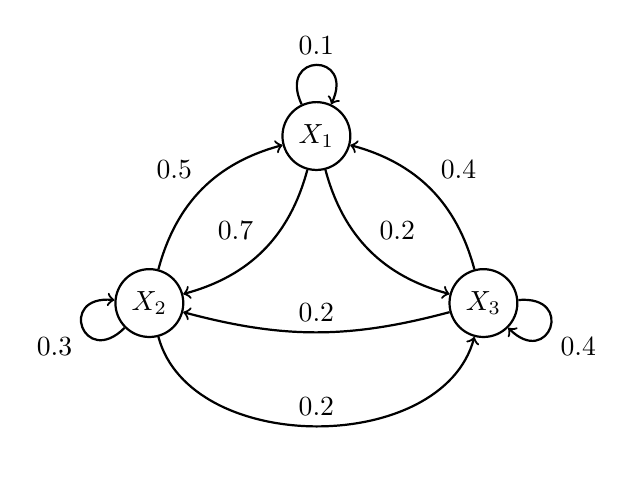
\begin{tikzpicture}[node distance={30mm}, thick, main/.style = {draw, circle}] 
    \node[main] (1) {$X_1$}; 
    \node[main] (2) [below left of=1] {$X_2$}; 
    \node[main] (3) [below right of=1] {$X_3$};
    \draw[->] (1) to [out=115,in=65,looseness=5] node[midway, above, pos=0.5] {0.1} (1);
    \draw[->] (1) to [out=-105,in=15,looseness=1] node[midway, above left, pos=0.5] {0.7} (2);
    \draw[->] (1) to [out=-75,in=165,looseness=1] node[midway, above right, pos=0.5] {0.2} (3);
    \draw[->] (2) to [out=75,in=195,looseness=1] node[midway, above left, pos=0.5] {0.5} (1);
    \draw[->] (2) to [out=225,in=175,looseness=5] node[midway, below left, pos=0.5] {0.3} (2);
    \draw[->] (2) to [out=285,in=255,looseness=1] node[midway, above, pos=0.5] {0.2} (3);
    \draw[->] (3) to [out=105,in=-15,looseness=1] node[midway, above right, pos=0.5] {0.4} (1);
    \draw[->] (3) to [out=195,in=-15,looseness=1] node[midway, above, pos=0.5] {0.2} (2);
    \draw[->] (3) to [out=5,in=-45,looseness=5] node[midway, below right, pos=0.5] {0.4} (3);
    \label{fig:sampleChain1}
    \end{tikzpicture}
    \caption{Ejemplo de una cadena de Markov} 
    \label{fig:sampleChain1}
    \end{figure}
    
    Internamente, las cadenas de Markov se suelen representar con matrices de transición, tales como la de la tabla \ref{tab:sampleChainMatrix}

    \begin{table}
	\centering
	\begin{tabular}{c|c|c|c}
		\textbf{} & \textbf{$X_1$} & \textbf{$X_2$} & \textbf{$X_3$}\\
		\hline
		\textbf{$X_1$} & 0.1 & 0.7 & 0.8\\
		\hline
		\textbf{$X_2$} & 0.5 & 0.3 & 0.2\\
		\hline
		\textbf{$X_3$} & 0.4 & 0.2 & 0.4\\
	\end{tabular}
	\caption{Ejemplo de una matriz de transición}
	\label{tab:sampleChainMatrix}
    \end{table}
    
    \subsection{Entrenamiento de las Cadenas de Markov}
    \label{subsec:entrenamientoCadenasMarkov}
    Una ventaja de las cadenas de Markov es su fácil entrenamiento. Una vez tenemos nuestro dataset limpio y normalizado (como se explica en \ref{sec:dataset}) podemos recorrerlo para construir la matriz de transición.

    En nuestro caso, cargamos todas las secuencias de notas del dataset, descartamos las notas que no tienen otra a continuación (serían las que se encuentran al final de la melodía) y rellenamos una tabla de ocurrencias con cada vez que una nota específica se encuentra después de otra.

    Por ejemplo, si hubieran sólo 4 notas (cabe destacar que las notas se encuentran en notación \textit{pitch\_duración}, dicha notación se explica en \ref{subsub:representacion-pitch_duracion}) podría quedar la matriz de ocurrencias dada en la tabla \ref{tab:sampleOcurrenceMatrix} tras recorrer todo el dataset.

    \begin{table}
	\centering
	\begin{tabular}{c|c|c|c|c}
		\textbf{} & \textbf{$60\_2$} & \textbf{$64\_1$} &         
            \textbf{$65\_2$} &     \textbf{$67\_1$}\\
		\hline
		\textbf{$60\_2$} & 238 & 119 & 280 & 63\\
		\hline
		\textbf{$64\_1$} & 120 & 50 & 185 & 145\\
		\hline
		\textbf{$65\_2$} & 117 & 108 & 15 & 60\\
		\hline
		\textbf{$67\_1$} & 120 & 20 & 36 & 24\\
	\end{tabular}
	\caption{Ejemplo de matriz de ocurrencia}
	\label{tab:sampleOcurrenceMatrix}
    \end{table}

    Posteriormente sumamos cada fila y convertimos a probabilidades cada entrada de la tabla dividiendo entre la suma de su fila. Con esto obtenemos una matriz de transición como la de la tabla \ref{tab:sampleTransitionMatrix}.

    \begin{table}
	\centering
	\begin{tabular}{c|c|c|c|c}
		\textbf{} & \textbf{$60\_2$} & \textbf{$64\_1$} &         
            \textbf{$65\_2$} &     \textbf{$67\_1$}\\
		\hline
		\textbf{$60\_2$} & 0.34 & 0.17 & 0.4 & 0.09\\
		\hline
		\textbf{$64\_1$} & 0.24 & 0.1 & 0.37 & 0.29\\
		\hline
		\textbf{$65\_2$} & 0.39 & 0.36 & 0.05 & 0.2\\
		\hline
		\textbf{$67\_1$} & 0.60 & 0.1 & 0.18 & 0.12\\
	\end{tabular}
	\caption{Ejemplo de matriz de transición calculada a partir de la matriz de ocurrencia}
	\label{tab:sampleTransitionMatrix}
    \end{table}

    Con la matriz de transición ya podríamos ejecutar la cadena de markov durante N iteraciones para obtener una melodía. En nuestro caso utilizamos la librería de Python PYDTMC, que proporciona modelos de markov ya implementados (para más información sobre dicha librería consultar \cite{PYDTMC}). Con esta librería podemos crear una cadena de Markov a partir de la matriz de transición y poder guardarla a archivo, ejecutar o bien N pasos o paso a paso y dibujarla con matplotlib.
    
    La representación gráfica de la cadena se puede ver en la figura \ref{fig:sampleNotesChain}.

    \begin{figure}
    \centering
    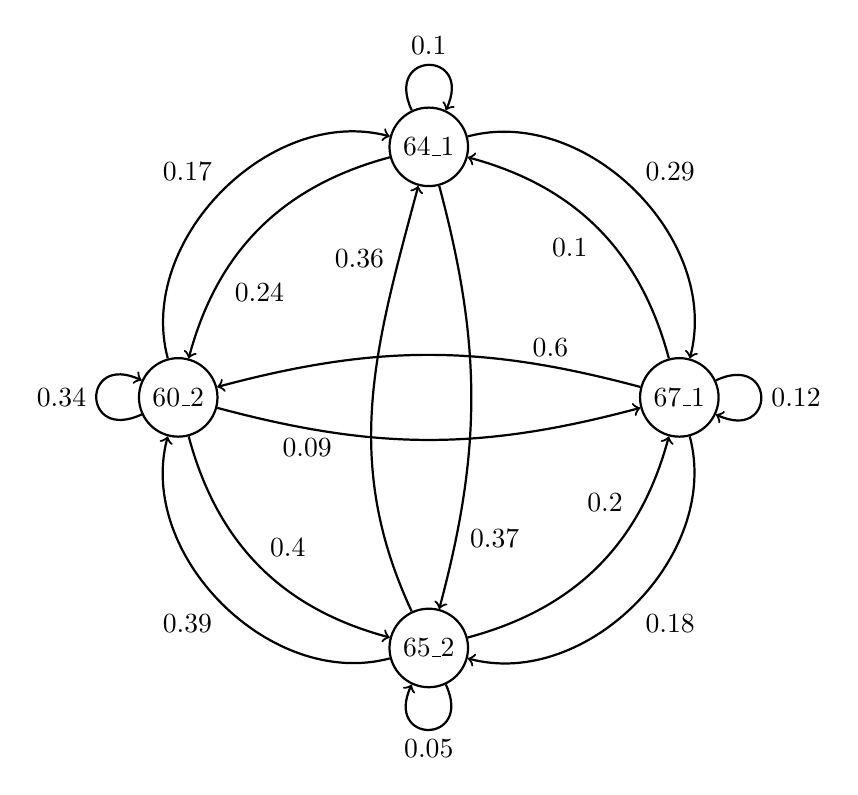
\begin{tikzpicture}[node distance={45mm}, thick, main/.style = {draw, circle}] 
    \node[main] (1) {$60\_2$}; 
    \node[main] (2) [above right of=1] {$64\_1$}; 
    \node[main] (3) [below right of=1] {$65\_2$};
    \node[main] (4) [below right of=2] {$67\_1$};
    \draw[->] (1) to [out=205,in=155,looseness=5] node[midway, left, pos=0.5] {0.34} (1);
    \draw[->] (1) to [out=105,in=165,looseness=1] node[midway, above left, pos=0.5] {0.17} (2);
    \draw[->] (1) to [out=-75,in=-195,looseness=1] node[midway, above right, pos=0.5] {0.4} (3);
    \draw[->] (1) to [out=-15,in=195,looseness=1] node[midway, below , pos=0.2] {0.09} (4);
    \draw[->] (2) to [out=195,in=75,looseness=1] node[midway, below right, pos=0.7] {0.24} (1);
    \draw[->] (2) to [out=115,in=65,looseness=5] node[midway, above, pos=0.5] {0.1} (2);
    \draw[->] (2) to [out=-75,in=75,looseness=1] node[midway, below right, pos=0.8] {0.37} (3);
    \draw[->] (2) to [out=15,in=75,looseness=1] node[midway, above right, pos=0.5] {0.29} (4);
    \draw[->] (3) to [out=195,in=255,looseness=1] node[midway, below left, pos=0.5] {0.39} (1);
    \draw[->] (3) to [out=115,in=255,looseness=1] node[midway, above left, pos=0.8] {0.36} (2);
    \draw[->] (3) to [out=295,in=245,looseness=5] node[midway, below, pos=0.5] {0.05} (3);
    \draw[->] (3) to [out=15,in=255,looseness=1] node[midway, above left, pos=0.7] {0.2} (4);
    \draw[->] (4) to [out=165,in=15,looseness=1] node[midway, above, pos=0.2] {0.6} (1);
    \draw[->] (4) to [out=105,in=-15,looseness=1] node[midway, below left, pos=0.5] {0.1} (2);
    \draw[->] (4) to [out=-75,in=-15,looseness=1] node[midway, below right, pos=0.5] {0.18} (3);
    \draw[->] (4) to [out=25,in=-25,looseness=5] node[midway, right, pos=0.5] {0.12} (4);
    \end{tikzpicture}
    \caption{Representación visual de la cadena obtenida a partir de la matriz de transición} 
    \label{fig:sampleNotesChain}
    \end{figure}

    \subsection{Generar melodías con Cadenas de Markov}
    \label{subsec:generarCadenasMarkov}
    Para crear melodías, podemos realizar el número de iteraciones que queramos sobre la cadena para crear una melodía de la longitud deseada, el acercamiento más simple sería generar N notas. 
    
    En nuestro generador (definido en markovGenerator.py) se puede especificar el número de steps deseado y se generarán iteraciones suficientes hasta llegar al límite. Al ejecutar comenzamos siempre en "C4\_2", por conveniencia.

    El modelo nos construye una melodía que posee cierta coherencia debido al entrenamiento, pero al existir aleatoriedad, es un modelo que no es determinista, por lo que cada melodía será distinta.

    \subsection{Puntos fuertes y débiles de la generación de melodías con Cadenas de Markov}
    \label{subsec:ventajasYDesventajasMarkov}
    Las cadenas de Markov resultan muy potentes como primer acercamiento, pues son un modelo simple y fácil de entender. El entrenamiento es sencillo y su ejecución una vez entrenada es prácticamente instantánea.

    Sin embargo, tienen algunas desventajas. Primero, hablando de rendimiento y escalabilidad, cada nodo de la cadena tiene que representar una nota con duración como mínimo, por lo que en la práctica se crea una cadena inmensa aunque limitemos a 2 octavas el posible rango melódico. Además, aunque la ejecución de pasos en la cadena sea instantáneo, el coste de cargarla y guardarla a archivo es muy grande, pudiendo tardar más de medio minuto.

    Además, desde el punto de vista musical, no proporcionan una melodía muy rica, ya que dependen completamente de la probabilística, las melodías generadas no tendrán una coherencia aparente. Aunque ese punto no resulta muy crítico para nuestro trabajo por el resto de etapas que realizamos, es conveniente obtener una melodía lo más agradable posible.

    Por estos inconvenientes, resulta interesante explorar otros modelos.

\section{Redes Neruonales Recurrentes}
\label{sec:RNR}

\section{Magenta}
\label{sec:magenta}